\begin{abstract}
A diagnostic action changes both what an autonomous robot knows and which task continuations remain possible. An informative contact may preserve conventional motion constraints yet remove an otherwise executable correction. We study this coupling in physics-based robotic simulation through \emph{post-diagnosis recoverability}, the set of fixed feedback corrections that complete the task within the remaining deadline. Our methodology combines a physical belief update, response-contingent recovery, and matched probe-versus-hold interventions that distinguish contact-induced option loss from elapsed time. We formulate two quantitative hypotheses: informative probing causes materially frequent recovery-option erasure, and modeling its consequences improves task completion relative to constrained information seeking. An exact finite-world illustration demonstrates the conflict; a prospective contact-rich assembly study specifies the probes, controls, recovery policies and statistical tests needed to establish its prevalence and consequences. The result is a testable methodology for judging diagnosis by both information gained and task recovery retained.
\end{abstract}



\section{Introduction}
Consider a simulated robot attempting an insertion when contact contradicts its expected alignment. A small physical probe can reveal an obstruction, but also wedge the part more tightly. Even inside workspace and contact limits, the robot may have fewer successful ways to finish. Contact-rich assembly makes this coupling consequential (Fig.~\ref{fig:concept}) \citep{tang2023,tao2025}.

Active perception uses action to improve observations \citep{bohg2017}; safe active diagnosis constrains exploratory motion \citep{ragan2024,sheng2024}. DA-GRD stops when pose hypotheses support a common executable grasp and explicitly models contact-induced object motion \citep{wang2026}. Task-compatible active calibration connects identification motions with finite-horizon downstream controllability \citep{kobayashi2026}; reversibility-aware learning values return paths \citep{grinsztajn2021}. Our specific estimand concerns \emph{postfailure, equal-time probe-versus-hold loss of a fixed feedback-recovery catalogue}. It asks which corrections cease to work because of diagnosis rather than mere delay, and whether predicting that contrast changes decisions beyond existing task-aware alternatives.

We develop a recoverability-preserving diagnosis (RPD) methodology: define success relative to task, repertoire and deadline; measure physical option changes against a matched hold; and compare decisions with and without predicted recovery consequences. Standard contingent planning supplies the mechanism \citep{sheng2024}, not a new solver. The scientific question is \emph{when does informative probing destroy recoverable continuations, and when does anticipating this loss improve completion?}

\textbf{H1, informative option erasure.} A frozen constrained information-gain (IG) selector produces constraint-compliant full-repertoire erasure in more than 10\% of predecision-eligible assembly checkpoints, counting direct action and abstention in the denominator. In over half of these erasure cases, the probe increases held-out likelihood of the original contact mode by more than 20\% over both initial and equal-duration-hold predictors.

\textbf{H2, decision consequence.} With identical observations, models, controls and time budgets, recoverability-aware selection increases terminal completion by more than five percentage points over constrained IG, while increasing whole-path violation risk by less than two points. The margins represent one compromised recovery per ten eligible attempts and one additional completion per twenty. These are prospective predictions, not observed effects. We expect contact-dependent losses near clearance-scale probing, not universal damage from information gathering.

\begin{figure}[t]
\centering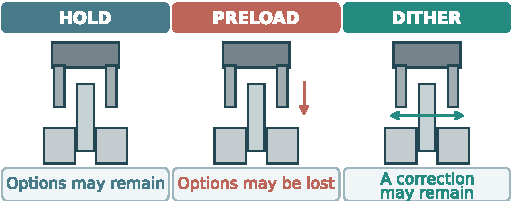
\includegraphics[width=\columnwidth]{figures/figure1.pdf}
\caption{\textbf{Why physical diagnosis can change recovery.} Holding, axial preload and lateral dither start from the same uncertain insertion condition but can leave different corrections available. This is conceptual, not a measured outcome. Equal-duration branches separate physical intervention effects from time; alternative futures are evaluated offline.}\label{fig:concept}
\end{figure}

\section{Problem: What Can Still Be Recovered?}
Let $s$ contain physical state, controller memory, random-generator state, task flag and clock. History $h$ induces belief $b(s\mid h)$ and support $\B(h)$. Fix two feedback corrections $\A=\{a_0,a_1\}$, remaining time $\tau$, and binary task completion $G(s,a,\tau)$. Define
\begin{equation}
\begin{split}
\K_\tau(s)&=\{a\in\A:G(s,a,\tau)=1\},\\
\operatorname{Common}_\tau(B)&=\bigcap_{s\in B}\K_\tau(s).
\end{split}\label{eq:set}
\end{equation}
Every plausible state can admit a correction while their intersection is empty: recoverability need not mean the robot knows which correction works. An empty set concerns only these policies and this deadline, not every possible robot skill. Longer time or another skill can restore an option.

A probe $p$ lasts $d_p$, physically transforms state by $T_p$, and returns $y=O_p(s,T_p(s),\xi_p(s))$ along trajectory $\xi_p$. Its compatible successor states are
\begin{equation}
 B_{p,y}=\{T_p(s):s\in\B(h),\ O_p(s,T_p(s),\xi_p(s))=y\}.
\end{equation}
In a complete deterministic reference model, a probe permits robust response-contingent recovery exactly when
\begin{equation}
 \forall y\text{ reachable},\quad \operatorname{Common}_{\tau-d_p}(B_{p,y})\ne\emptyset.
 \label{eq:robust}
\end{equation}
Necessity follows because one correction must work for all states compatible with each response; sufficiency follows by selecting one member of each intersection. The transformation precedes recovery: merely partitioning the original state would ignore physical damage. For stochastic dynamics, a joint transition--observation kernel replaces $T_p,O_p$; Eq.~\eqref{eq:robust} then applies to its declared robust support, not automatically to physical uncertainty or a calibrated success probability.

Probabilistic selection uses the standard one-probe value
\begin{equation}
 V(p\mid b,\tau)=\E_{y\mid p,b}\!\left[\max_{a\in\A}\E_{s'\mid y,p,b}\widehat G(s',a,\tau-d_p)\right],
 \label{eq:value}
\end{equation}
compared with direct correction and STOP. The fitted model is discovery-frozen. IG instead maximizes predicted contact-mode information under the same modeled pre-recovery constraint gate. Both use the executed response to choose a correction; neither receives alternative future outcomes online. Both first recover directly if the model supplies a common successful correction. A full-model planner with Eq.~\eqref{eq:value} is an equivalence control, not an opponent expected to lose. Exact reference-model planning and prediction error in physical contact remain separate questions.

\section{Methodology: Separate Learning from Losing Options}
\subsection{The matched physical measurement}
Comparing success before and after a probe confounds state change with elapsed time. From the same qualified checkpoint, compare $T_p$ with an equal-duration commanded hold $H_{d_p}$. Hold maintains equilibrium and feedback gains while gravity, time and contact dynamics continue. Execute each fixed correction after both branches with budget $\tau-d_p$ (Fig.~\ref{fig:protocol}). Full-repertoire erasure is
\begin{equation}
 L_p(s)=\ind[\K_{\tau-d_p}(H_{d_p}(s))\ne\emptyset\ \land\ \K_{\tau-d_p}(T_p(s))=\emptyset].
 \label{eq:loss}
\end{equation}
Removing $a_0$ while $a_1$ survives is an individual-option loss, not $L_p$. Also record option creation. Let $C_p,C_H$ indicate measured probe/hold path compliance and $J_p=L_pC_pC_H$. The primary prevalence is
$q_{\rm IG}=\E_{s\sim\mathcal D_{\rm eligible}}J_{\pi_{\rm IG}(h(s))}(s)$.
Direct action and STOP contribute zero \emph{probe-induced erasure} but stay in the denominator; their terminal outcomes are never imputed. Report probe-selection rate $\rho_{\rm IG}$, hold-recoverable fraction $\rho_H$, fixed-probe $q_p=\Pr(J_p=1)$ over every eligible parent, and $q_{\rm IG}/\rho_H$ when $\rho_H>0$.

Simulator replay supplies isolated alternative branches; the acting policy follows only one. Root/controller/clock parity is required, with no reset between probe and correction. Loss is catalogue- and time-relative. Enlarging the repertoire may create or remove this comparative event because both hold and probe success can change. Primary $\K$ is goal-based; additionally report $\K^C$ requiring compliant recovery. Probe compliance alone is not safe task completion.

\begin{figure*}[t]
\centering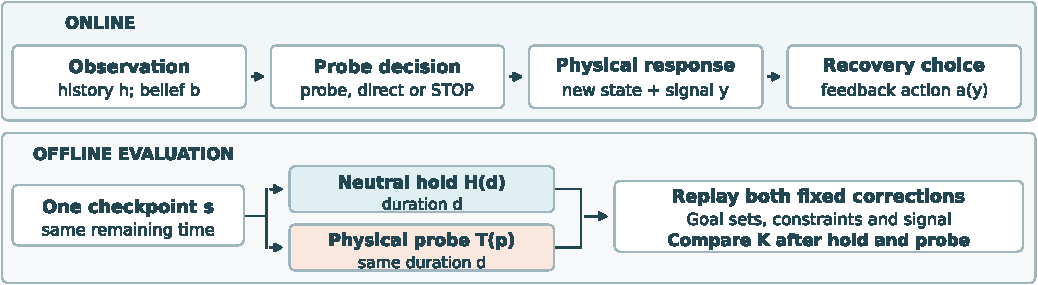
\includegraphics[width=\textwidth]{figures/figure2.pdf}
\caption{\textbf{One simulated decision, matched offline measurement.} Online, history selects a probe, direct action or STOP; the executed response informs one correction. Offline replay compares equal-duration hold and probe at the same checkpoint, each followed by both fixed corrections. Paired alternatives, latent mode and true object pose are never available to the acting policy.}\label{fig:protocol}
\end{figure*}

\subsection{Was the probe genuinely informative?}
Let $Z$ be the original pre-probe contact mode, $X$ the root features, and $Y_p,Y_H$ the probe/hold responses. Discovery-trained, frozen predictors $f_0(Z\mid X)$, $f_p(Z\mid X,Y_p)$ and $f_H(Z\mid X,Y_H)$ give
\begin{equation}
 \begin{split}D_0&=\log f_p(Z)-\log f_0(Z),\\D_H&=\log f_p(Z)-\log f_H(Z).\end{split}
\end{equation}
With $\gamma=\ln1.2$, set $M_{p,\gamma}=\ind[D_0>\gamma\land D_H>\gamma]$. H1 requires $q_{\rm IG}>.10$ and $\eta_\gamma=\Pr(M_{p,\gamma}=1\mid J_p=1)>.50$, where $p$ is IG-selected. Thus diagnostic signal and erasure must occur in the same cases. At a uniform three-mode prior, 20\% greater likelihood raises the true-mode probability from $1/3$ to above $.4$; the majority criterion is neither universal chance level nor positive mean information. Report score means and joint prevalence $q_{\rm IG}\eta_\gamma$. A response shuffle within discovery-frozen root strata checks dependence on the measured signal; comparable shuffled gains defeat a useful-signal interpretation. Zero erasures leave $\eta_\gamma$ undefined.

\subsection{Does preserving options improve decisions?}
For terminal indicator $U$ and whole-postroot-path violation $V_C$, H2 concerns paired-parent effects
\begin{equation}
 \begin{split}\Delta_U&=\E[U(\pi_{\rm RPD})-U(\pi_{\rm IG})],\\
 \Delta_C&=\E[V_C(\pi_{\rm RPD})-V_C(\pi_{\rm IG})].\end{split}
\end{equation}
H2 requires $\Delta_U>.05$ and $\Delta_C<.02$, regardless of H1. A response-blind rule on the same post-probe state isolates information's decision value; direct recovery tests whether probing was needed. Task consensus and full-objective planning share transitions and terminal objectives and may equal RPD exactly. Report equality, completion, information, invocation counts, time, commanded motion, option changes, violations and prediction error separately. H2 gain may reflect saved probe time or action choice, not causal mediation by erasure alone; invocation counts do not establish energy savings.

\section{Proposed Simulation Study: Contact-Rich Assembly}
\subsection{Checkpoint population, controls and outcomes}
Use pinned ManiSkill3~3.0.1/SAPIEN~3.0.3, CPU PhysX, Panda native absolute \emph{pd\_ee\_pose}, 100\,Hz physics and 20\,Hz control \citep{tao2025}. These are proposed study settings, not qualified tolerances. Native square peg half-length $\ell\sim U[85, 125]$\,mm, half-width $r\sim U[15, 25]$\,mm and per-side clearance $c=3$\,mm are retained. Public hole frame $H$ has world position $(.05,.30,.15)$\,m, identity rotation; $+x$ is insertion. Nominal peg centre is $(-2\ell-2c, 0, 0)$ in $H$, with identity orientation; TCP is 60\,mm behind it with $R_x(\pi)$ orientation. Native peg/fixture friction $.3/.3$, finger friction $2/2$ and zero restitution are unchanged.

Draw three equally probable hidden modes: $y$ offset $\pm1.25c$ with $z\sim U[-c/4,c/4]$; the exchanged $z$ mode; or transverse offsets in that box and one equiprobable pitch/yaw offset $\pm2\theta_c$, $\theta_c=\arctan(c/(2\ell))$. Signs are fair. Errors change the actual peg-in-tool transform; no exact object pose is exposed online. Initialize zero velocities and native IK (100 iterations), seeded by $(0,\pi/8,0,-5\pi/8,0,3\pi/4,-\pi/4)$ with fingers at 40\,mm. Require IK residuals $c/10,\theta_c/10$. After this initialization-only placement, close the grasp for $.5$\,s and command a $3c$ approach over 1\,s, without welding or subsequent state reset. Native stiffness/damping/effort limits remain $1000/100/100$, in Nm/rad,Nm\,s/rad,Nm for joints and N/m,N\,s/m,N for fingers. Eligibility requires no goal, native two-finger grasp, finite healthy controller state, contact $\ge.5$\,N throughout the last $.05$\,s, and TCP residual $[c/4, 4c]$ within the constraints below. Selection uses only predecision source checks, never candidate probe/recovery outcomes. All attempted parents and exclusions remain recorded. This conditional population is not all robot failures; unique seeds do not prove IID sampling.

Over $d=.5$\,s (ten updates), hold retains equilibrium $u_0$; preload commands $u_0+(c/2)(3v^2-2v^3)e_x$, $v=k/10$; dither commands $u_0+c\sin(2\pi k/10)e_y$, with its final command exactly $u_0$. Orientation and gripper commands stay fixed. Equal commanded endpoint does not imply equal physical state. Primary remaining budget is $\tau=4$\,s, leaving 3.5\,s after intervention; direct recovery has 4\,s. Native clock and controller memory persist, and both wrappers allow 200 updates.

Both feedback macros target peg head $(-10, 0, 0)$\,mm in $H$, identity orientation. Policy $a_0$ inserts from nominal grasp calibration in 40 updates then holds. Policy $a_1$ withdraws $4c$ in ten, realigns to head $(-\ell-2c,0,0)$ with identity orientation in ten, reinserts in forty, then holds, using a root-fitted grasp transform computed once and shared across every branch. From measured macro-start TCP then commanded segment endpoints, interpolate $3v^2-2v^3$ translation and shortest-path rotation. Responses choose a macro, not privileged new execution parameters.

Success is stable held mid-depth insertion: head $x\in[-15, 15]$\,mm, centre $|y|,|z|\le c/2$, orientation error $\le\theta_c$, linear/angular speed $\le c$/s and $\theta_c$/s for 26 consecutive 100\,Hz samples spanning $.25$\,s. Keep monitoring after the first success to the deadline. The native head-only flag is secondary. At every substep check native joint limits, arm speed $\le2$\,rad/s, TCP residual $\le4c$, grasp slip translation/rotation $\le c, 2\theta_c$, peg--fixture net force $\le10m_{\rm peg}g$, and nonfinger robot contact with peg/fixture $\le.5$\,N. Violations stay measured outcomes, not exclusions. These sampled simulation envelopes are not continuous-time or hardware safety guarantees.

Online $X$ has 28 scalars: seven arm positions/velocities, calibrated TCP position/rotation-log, commanded position/rotation-log and $\ell,r$. Each response tick has 23: arm positions/velocities, TCP pose and tracking-position residual. Ten ticks give 230 dimensions. True peg pose, mode, grasp error, contact force and alternative outcomes remain evaluator-only; no force/aperture sensor is invented.

\subsection{Frozen shared model and qualification}
Use 384 independently eligible discovery parents: 256 fit and 128 disjoint predictor audit; five-fold parent-grouped CV stays within fitting. Fit the root grasp transform from fitting-root features and evaluator training labels, then freeze it before outcome collection. Normalize metric quantities by $c$, rotations by $\theta_c$, and joints/rates by 1\,rad and 1\,rad/s; fitting means and standard deviations (floored at 1) set the final scale. Fixed calibration weights are $w_i^E\propto\exp[-\|X-X_i\|^2/(2d_X)]$, $d_X=28$. Average translations and sign-aligned unit quaternions, renormalizing; a quaternion norm below $10^{-8}$ uses the first fitting ID. Use that same root estimate for every matched branch; later prediction tuning never changes executed macro parameters.

Reference particles store $X_i,Y_{ip}$, source mode and continuation labels. Model root weights are $w_i\propto(w_i^E)^{1/b_X^2}$. For each probe or hold, the finite response channel is $P_p(j\mid i)\propto\exp[-\|Y_{jp}-Y_{ip}\|^2/(2b_Y^2d_Y)]$, normalized over fitting codewords $j$, $d_Y=230$. A measured response maps to the nearest codeword, ties by ID; Bayes weights $w_iP_p(j\mid i)$ predict both mode and continuation success. Per-particle macro outcomes are independent of codeword because execution parameters were fixed at the root. IG computes mutual information about $Z$ in this channel; RPD uses Eq.~\eqref{eq:value}. Both gate probes by $\sum_iw_i(1-C_{ip})\le.02$. These fitted probabilities are not calibrated physical safety guarantees.

Bandwidths are chosen from $\{1/2, 1, 2, 4\}$ by grouped log-score CV, then frozen; independent audit never refits them. Smooth each three-mode prediction by $(1-3\epsilon)f+\epsilon$, $\epsilon=.001$. Ties prefer shorter duration, less commanded motion, then ID. STOP uses the actual prefix goal/violation flags. A root-common successful correction takes precedence for both selectors; otherwise IG selects its qualifying probe, falling back to best direct expected success or STOP. The reference planner and Bayesian task-consensus adaptation use the same value and tie rules, preserving equivalence rather than claiming native DA-GRD reproduction.

The \emph{technical} predictor gate requires intact source/mode labels, complete 23-channel ten-tick responses, finite normalized probabilities, no evaluator leakage, and at least 20 audit parents of each original mode. An independent synthetic known-signal control carries a balanced three-mode code through the same response-processing/classification interface; require at least 116/128 correctly decoded, with one-sided 95\% CP lower $>.80$. This tests the pipeline, not actual probe information gain. Neither high real-probe informativeness, erasure nor positive H2 is a gate. Audit proper log score, calibration and shuffle sensitivity without accepting only favorable real-probe responses.

Source qualification is separate: first demonstrate nominal compliant insertion and successful postfailure recovery after neutral holding; then freeze a new source and 12 disjoint qualification seeds. Require at least eight eligible and six post-hold-recoverable roots, finite legal channels, and replay parity in body/joint state, drive targets, commands, estimator, clock and goal dwell ($10^{-5}$\,m/$10^{-4}$\,rad pose tolerances). An earlier technical source yielded 7/12 eligible, 0/49 distinct terminal goals and 0/49 whole-path compliant branches, with 14 replay repeats. Its empty hold repertoire is a source limitation, not a test of H1 or a benign-probe finding. A failed gate stops the campaign without replacement seeds or relaxed thresholds.

\subsection{Independent evaluation and statistical decisions}
Dose response uses 64 additionally disjoint parents, not confirmation tuning. Candidate caps are 768 discovery, 128 dose and 2560 confirmation, with all failures/exclusions retained. Register disjoint ordered parent lists before collection. Freeze source, models, selectors and ties before screening 1024 eligible confirmation parents, then open outcomes. Hold, preload and dither followed by both macros cost 6144 terminal continuations, plus one shared direct-policy control per parent. Branches and repeats never increase independent $n$. Every regenerated root must match its fingerprint; missing outcomes are unavailable, not failed tasks or zero events.

For explicit resource accounting, discovery collects the six matched branches plus both full-deadline direct macros: $384\times8=3072$ labels. The 64 dose parents each supply hold and both probes at three amplitudes followed by both macros: $64\times14=896$. Confirmation requires $1024\times7=7168$, totaling 11136 terminal episodes before screening, qualification and replay checks. A doubled-deadline six-branch comparison on the same 64 dose parents adds 384, totaling 11520; an unavailable extra skill is excluded. Source-qualified timings must establish feasibility before confirmation. Parallelization uses fresh isolated processes, never correlated branches as extra parents. If the fixed budget cannot be completed, retain the atomic parent, unfinished IDs and missingness; never reduce margins or choose effect-rich replacements.

H1 uses one-sided exact Clopper--Pearson (CP) lower bounds \citep{clopper1934} for $q_{\rm IG}>.10$ and $\eta_\gamma>.50$, each at $.025$, with conditional-binomial inference given the random erasure count under independent parents and frozen models. The conjunction is an intersection--union test. Report $\rho_{\rm IG},\rho_H,q_p$ and $q_{\rm IG}/\rho_H$; low selected-policy erasure does not establish both probes benign. Limited fixed-probe claims require simultaneous upper bounds, $.0125$ per probe. For $k$ observed events and $b$ missing binary labels in $n$, report $[L(k,n),U(k+b,n)]$. For conditional signal, take the envelope of CP intervals over all admissible assignments of missing erasure membership and signal labels; if an assignment permits zero erasures, no unconditional positive $\eta_\gamma$ claim is made.

For H2 completion, let $n_+,n_-$ count RPD-only and IG-only successes, $m=n_++n_-$, $r=\Pr(U_{\rm RPD}\ne U_{\rm IG})$, and $\theta=\Pr(U_{\rm RPD}=1\mid U_{\rm RPD}\ne U_{\rm IG})$. Then $\Delta_U=r(2\theta-1)$. Allocate $.0125$ to each one-sided CP bound: multiply $2L(\theta)-1$ by $L(r)$ when nonnegative, otherwise $U(r)$; at $m=0$ use $-U(r)$. This gives a valid 97.5\% lower bound.

For RPD-only/IG-only violations $v_+,v_-$, set $m_C=v_++v_-$, $\epsilon_C=.02$ and
\begin{equation}
 Z_C=\frac{v_+-v_--n\epsilon_C}{\sqrt{n[\max(m_C/n,\epsilon_C)-\epsilon_C^2]}}.
\end{equation}
Under $\Delta_C\ge\epsilon_C$, the rejection probability is bounded on the boundary $\Delta_C=\epsilon_C$ over discordance $r_C\in[\epsilon_C, 1]$, with probabilities $(r_C\pm\epsilon_C)/2$. For $n=1024$, $Z_C\le-2.2$ has size at most $.023485663<.025$, certified over the continuum by 1025 nonnegative Bernstein coefficients. This is a conservative finite-sample bound, not an asymptotic score claim. H2 needs both lower$(\Delta_U)>.05$ and this violation rejection. With missing pairs, envelope completion bounds over all admissible paired labels and require violation rejection for every admissible count completion; complete-case selection is invalid.

If screening reaches 2560 candidates with fewer eligible parents, register realized $n$ and independently recalibrate the composite-null critical \emph{before inspecting confirmation outcomes}. Do not reuse the 1024 critical or power, impute parents, or drop source-invalid labels. Each endpoint concerns independent parents conditional on the frozen source and discovery model.

At 1024 parents, 123 erasures clear the prevalence test; zero events give a97.5\% upper $.00359594$. At hypothetical $q=.15,\eta=.80$, H1 joint power is $.9974$. Completion discordance $.20$ with gain $.12$, and violation discordance $.025$ with zero difference, give H2 component powers $.9926,.9637$, hence joint power at least $.9563$ regardless of endpoint dependence. These are design alternatives, not robot outcomes.

\begin{table}[t]\centering
\caption{Matched outcomes distinguish competing explanations.}\label{tab:controls}
\begin{tabular}{p{.32\columnwidth}p{.58\columnwidth}}\toprule
Pattern & Scoped interpretation\\\midrule
Hold and probe both fail & No demonstrated probe-specific erasure; catalogue or deadline can be inadequate.\\
Hold retains, probe loses all & Full-catalogue physical loss beyond waiting, under these macros and deadline.\\
Loss without mode signal & Disturbance, not H1 informative erasure.\\
H1 without H2 gain & A mechanism without the specified added policy benefit.\\\bottomrule
\end{tabular}
\end{table}

\section{Analytical Illustration and Scientific Implications}
Three equiprobable contact states $A,B,C$ admit $a_0$ in $A,B$ and $a_1$ in $C$. A fine probe reveals the mode ($\ln3=1.099$\,nats) but physically transforms $C$ so neither correction works. A coarse probe reveals $\{A,B\}$ versus $C$ ($.637$\,nats), preserves both states' corrections, and completes every task by choosing $a_0$ or $a_1$. Give both probes and hold equal duration, with nominally allowed paths. Fine achieves $2/3$, coarse $1$: more information can preserve physical constraints yet reduce task feasibility. This is an analytical construction, not simulation evidence or a new planning theorem; same-objective contingent planning equals RPD.

For a transparent constructed intensity sweep, split each mode into two equiprobable identical subtypes. Fine erases zero, one or both $C$ subtypes at intensities $.2,.5,.8$; hold and coarse preserve them. Erasure is then $0, 1/6, 1/3$, fine completion $1, 5/6, 2/3$, and coarse/RPD completion $1$. Table~\ref{tab:finite} makes this arbitrary finite transition schedule explicit; it is not a measured physical dose response.

\begin{table}[t]\centering
\caption{Exact constructed-model outcomes, not simulator measurements.}\label{tab:finite}
\begin{tabular}{cccc}\toprule
Intensity & Fine erasure & IG success & RPD success\\\midrule
$.2$ & $0$ & $1$ & $1$\\
$.5$ & $1/6$ & $5/6$ & $1$\\
$.8$ & $1/3$ & $2/3$ & $1$\\\bottomrule
\end{tabular}
\end{table}

\textbf{What is guaranteed?} Equation~\eqref{eq:robust} gives exact feasibility only inside the specified complete model. In contrast, confirmation bounds evaluate the frozen physical policies without assuming that their learned Bayes model is correct: valid source reconstruction and independent, stationary eligible-parent sampling suffice for the binary population inference. Model misspecification can reduce performance and falsify H2 while the statistical comparison remains valid. A source-invalid continuation instead lacks an outcome and enters missingness analysis. Neither uncertainty can be repaired by reporting a nominal planner optimum as a robot result.

The matched intervention controls the clock, initial physical state and controller memory, but does not make probing non-disturbing. Different contact, slip and feedback trajectories are precisely part of the declared intervention effect. A weaker observation model must not silently change the corrective controller: freezing the root transform and shared macro parameters separates catalogue selection from privileged post-probe execution. Offline matched futures are an evaluation instrument, not extra online attempts. At deployment both selectors share the four-second budget even though evaluating their counterfactual branches costs additional simulator executions.

\textbf{Catalogue and population scope.} Although $\K$ grows when a skill is added, erasure $L_p$ need not decrease: a new skill may succeed after hold only, creating a previously absent contrast, or after the probe, removing it. Similarly, the same probe can look destructive under a short deadline and recoverable under a longer one. The fixed primary catalogue and deadline make these comparisons interpretable; the secondary studies diagnose their dependence rather than establish universal viability. Original-mode prediction is evidence of diagnostic signal, not identification of a hidden causal damage mechanism. The shuffle is a sensitivity, not a calibrated randomization test without conditional exchangeability.

The physical study separately tests three frozen intensities $c/2,c, 3c/2$ and a doubled deadline on the disjoint dose cohort. These sensitivities do not alter primary policies or select favorable evaluation subsets. An extra-skill sensitivity remains unavailable unless a named fixed policy is independently qualified before confirmation; it cannot be invented after primary results. Completion, measured compliance, diagnostic signal and prediction error must be interpreted together.



The matched controls (Table~\ref{tab:controls}) separate these interpretations. H1 with no H2 benefit can mean information-driven loss is real but task consensus already handles it, or prediction error defeats planning. H2 without full erasure can reflect individual-option changes or direct-action timing. High fixed-probe $q_p$ but low $q_{\rm IG}$ means the selector avoids disruptive probes. Narrow simultaneous low $q_p$ bounds delimit these probes in this declared population; a wide interval, poor signal or unqualified source leaves a different question unresolved. Recovery after more time or a larger catalogue narrows the loss to deadline or repertoire, not universal irreversibility. A later independently sampled contact-task replication can test transport; it is not required to define this simulation-only methodology.

Our contribution is the recovery-specific matched intervention and its falsifiable population consequences. It does not claim a uniquely capable optimizer, hardware safety or an empirically established assembly effect. Even a precise negative result can determine where modeling physical diagnostic consequences is unnecessary within the tested scope; failed source qualification cannot supply that conclusion.
